\documentclass[11pt,a4paper]{article}
\usepackage[T1]{fontenc}
\usepackage[utf8]{inputenc}
\usepackage{lmodern}
\usepackage{amsmath,amssymb,amsthm,mathtools,mathrsfs}
\usepackage{graphicx,float,xcolor,multicol}
\usepackage[shortlabels]{enumitem}
\usepackage[margin=27mm]{geometry}
\usepackage{microtype,needspace,placeins}
\usepackage{tikz,tikz-cd}
\usetikzlibrary{arrows.meta,calc,positioning,patterns,decorations.pathreplacing}
\usepackage[colorlinks=true,linkcolor=teal,urlcolor=teal,citecolor=teal]{hyperref}
\setlength{\parindent}{0pt}
\setlength{\parskip}{.6em}
\setcounter{secnumdepth}{0}
\allowdisplaybreaks
\raggedbottom
\providecommand{\cross}{\times}
\DeclareUnicodeCharacter{2020}{\ensuremath{\dagger}}
\DeclareMathOperator{\supp}{supp}
\DeclareMathOperator*{\esssup}{ess\,sup}
\providecommand{\chapter}{\section}
\newenvironment{tool}[2]{\subsection*{Tool #1 --- #2}}{}
\newcommand{\ToolRef}[1]{Tool #1}
\newcommand{\FigureTag}[2]{\textit{Figure #1}}
\newcommand{\Result}[1]{\subsection*{#1}}
\newcommand{\Application}[1]{\subsubsection*{Application\if\relax\detokenize{#1}\relax\else\space--- #1\fi}}
\newcommand{\ProofHeading}{\par\textit{Proof.}\space}
\newcommand{\ProofOf}[1]{\par\textit{Proof of #1.}\space}
\newcommand{\RemarkHeading}{\par\textbf{Remark.}\space}
\newcommand{\NoteHeading}{\par\textbf{Note.}\space}
\newcommand{\ExerciseHeading}{\par\textbf{Exercise.}\space}

% Rendering support only; mathematical text is in each independent post.
\usepackage{booktabs,array,longtable}
\definecolor{HandoutBlue}{HTML}{2F6690}
\definecolor{HandoutNavy}{HTML}{17365D}
\newtheorem{theorem}{Theorem}
\newtheorem{lemma}[theorem]{Lemma}
\newtheorem{proposition}[theorem]{Proposition}
\newtheorem{corollary}[theorem]{Corollary}
\newtheorem{conjecture}[theorem]{Conjecture}
\newtheorem{definition}{Definition}
\newtheorem{example}{Example}
\newtheorem{namedtoolcounter}{Tool}
\newenvironment{namedtool}[1]{\begin{namedtoolcounter}[#1]}{\end{namedtoolcounter}}
\newtheorem*{claim}{Claim}
\newtheorem*{remark}{Remark}
\newtheorem*{exercise}{Exercise}
\newtheorem*{question}{Question}
\newtheorem*{observation}{Observation}
\newcommand{\SourceChapter}[2]{\section*{#2}}
\newcommand{\Lecture}[2]{\section*{Lecture #1: #2}}
\newcommand{\unclear}[1]{\textit{[unclear: #1]}}
\newcommand{\sourcegap}{\textit{[unfinished in the source]}}
\DeclareMathOperator{\dist}{dist}
\DeclareMathOperator{\id}{id}
\DeclareMathOperator{\Hol}{Hol}
\DeclareMathOperator{\Per}{Per}
\DeclareMathOperator{\Fix}{Fix}
\DeclareMathOperator{\diam}{diam}
\DeclareMathOperator{\Var}{Var}
\DeclareMathOperator{\Leb}{Leb}
\DeclareMathOperator{\Hom}{Hom}
\DeclareMathOperator{\End}{End}
\DeclareMathOperator{\Ann}{Ann}
\DeclareMathOperator{\Spec}{Spec}
\DeclareMathOperator{\Max}{Max}
\DeclareMathOperator{\Ob}{Ob}
\DeclareMathOperator{\Tor}{Tor}
\DeclareMathOperator{\Ass}{Ass}
\DeclareMathOperator{\Mor}{Mor}
\DeclareMathOperator{\Fun}{Fun}
\DeclareMathOperator{\Nat}{Nat}
\DeclareMathOperator{\Cone}{Cone}
\DeclareMathOperator{\MCG}{MCG}
\DeclareMathOperator{\Aut}{Aut}
\DeclareMathOperator{\Deck}{Deck}
\DeclareMathOperator{\SL}{SL}
\DeclareMathOperator{\PSL}{PSL}
\DeclareMathOperator{\Area}{Area}
\DeclareMathOperator{\im}{im}
\DeclareMathOperator{\PSh}{PSh}
\newcommand{\CRing}{\mathsf{CRings}}
\newcommand{\AMod}{A\text{-}\mathsf{Mod}}
\newcommand{\Ab}{\mathsf{Ab}}
\newcommand{\Z}{\mathbb Z}
\newcommand{\Q}{\mathbb Q}
\newcommand{\R}{\mathbb R}
\newcommand{\C}{\mathbb C}
\newcommand{\N}{\mathbb N}
\newcommand{\kk}{\mathbb k}
\renewcommand{\aa}{\mathfrak a}
\newcommand{\bb}{\mathfrak b}
\newcommand{\pp}{\mathfrak p}
\newcommand{\qq}{\mathfrak q}
\newcommand{\mm}{\mathfrak m}
\newcommand{\nn}{\mathfrak n}
\newcommand{\rad}{\mathrm r}
\newcommand{\cat}[1]{\mathsf{#1}}
\setcounter{secnumdepth}{0}
\allowdisplaybreaks

\graphicspath{{figures/miscellaneous/}}
\begin{document}
\section*{Flat Structures and Teichmüller Curves}
% BLOG-CONTENT-BEGIN
\subsection{Teichm\"uller Curves}
% Source page 1
Let $T_g$ denote the Teichm\"uller space of closed genus-$g$ surfaces.
We have the well-known identification $M_g\approx T_g/\MCG(g)$.
The action $\MCG(g)\curvearrowright T_g$ is properly discontinuous.
Consequently $M_g$ is a complex orbifold of dimension $3g-3$.
\setcounter{definition}{3}\begin{definition}[Teichm\"uller curve]
We say that $V\subset M_g$ is a Teichm\"uller curve if the inclusion
$(V\cong\mathbb H/\Gamma)\hookrightarrow M_g$ is an isometry. Its image lies in the regular locus. On $V$ we have the usual hyperbolic
metric coming from a torsion-free discrete subgroup
$\Gamma\subset\PSL_2(\mathbb R)$.
\end{definition}
\begin{question}
How do we get a metric on $M_g$?
\end{question}
\begin{figure}[H]
 \centering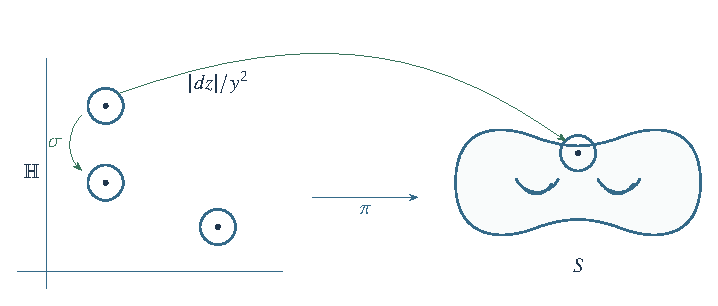
\includegraphics[width=.82\textwidth]{m3-fig-01.pdf}
 \FigureTag{M3.1}{fig:m3-fig-01}
\end{figure}
Here $\sigma\in\Deck(\mathbb H/S)<\Aut(\mathbb H)$.
% Author check: the metric label in the source is |dz|/y^2.
% Source page 2
One obtains a metric on $M_g$ in a similar fashion.
\begin{figure}[H]
 \centering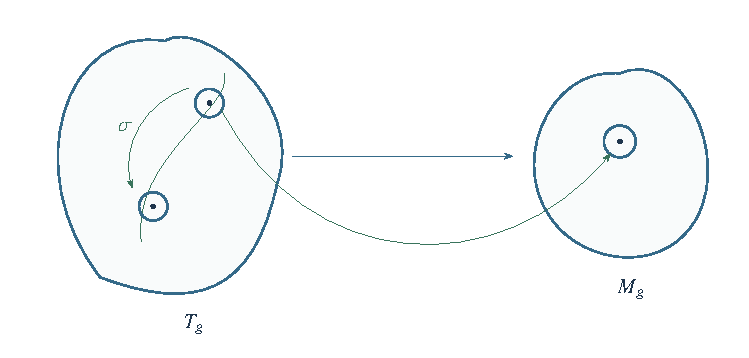
\includegraphics[width=.79\textwidth]{m3-fig-02.pdf}
 \FigureTag{M3.2}{fig:m3-fig-02}
\end{figure}

On $T_g$ one has the Weil--Petersson metric $\omega_{\mathrm{WP}}$.
\begin{enumerate}
 \setcounter{enumi}{0}\item The symplectic form is
 $\operatorname{Im}(\widetilde\omega_{\mathrm{WP}})
 =\sum_{i=1}^{3g-3}d\ell_i\wedge d\theta_i$.
 \begin{figure}[H]
  \centering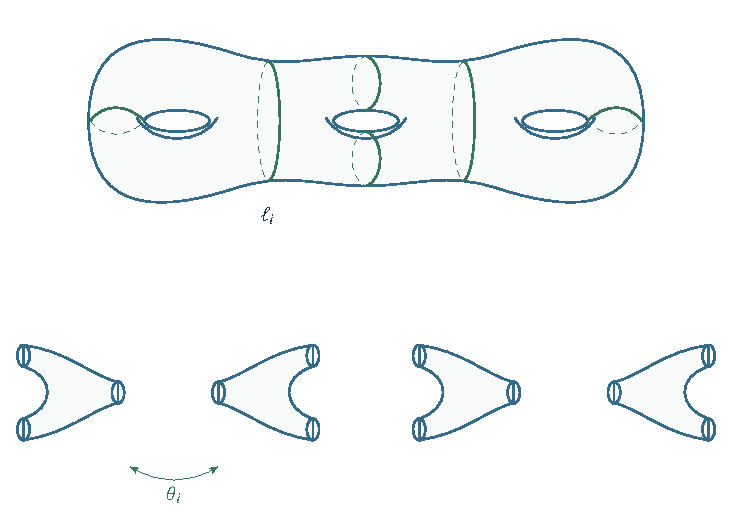
\includegraphics[width=.88\textwidth]{m3-fig-03.pdf}
  \FigureTag{M3.3}{fig:m3-fig-03}
 \end{figure}
 \setcounter{enumi}{1}\item $\widetilde\omega_{\mathrm{WP}}$ is a Hermitian form on $T_g$.
 We have $T_X(T_g)\approx\mathbb C^{3g-3}$ and
 $T_g\hookrightarrow\mathbb C^{3g-3}\ (Q^2(S_g))$. Set
 \[
  \langle q_1,q_2\rangle:=\int_X\frac{q_1\overline{q_2}}{\lambda^2},
 \]
 where $\lambda$ is the hyperbolic metric on $X$.
\end{enumerate}
% Source page 3
The real part $\operatorname{Re}(\widetilde\omega_{\mathrm{WP}})$ is a
Riemannian metric on $T_g$, and its imaginary part is a symplectic form
on $T_g$. Together they give a K\"ahler structure on $T_g$.
\setcounter{theorem}{6}\begin{theorem}
$\operatorname{Isom}_{\mathrm{WP}}(T_{g,n})=\MCG(g,n)$.

\end{theorem}
% Author check: the theorem attribution and WP designation are retained.
We do not need the full power of the theorem above to get a metric on
$M_g$. Let $\sigma\in\MCG(g)$. For $x=(S,f_1)$ and $y=(S,f_2)$, we have
\[
 d(\sigma\cdot x,\sigma\cdot y)=d(x,y)
 =\inf_{f\in[(f_2\circ\sigma)\circ(f_1\circ\sigma)^{-1}]}\ln K(f)
 =\inf_{f\in[f_2\circ f_1^{-1}]}\ln K(f).
\]
\begin{figure}[H]
 \centering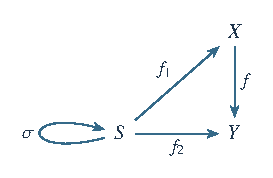
\includegraphics[width=.32\textwidth]{m3-fig-04.pdf}
 \FigureTag{M3.4}{fig:m3-fig-04}
\end{figure}
Thus $\sigma$ is distance-preserving and bijective. By the Myers--Steenrod
theorem, $\sigma$ preserves $\operatorname{Re}(\widetilde\omega_{\mathrm{WP}})$.
Here $d$ is the distance induced by
$\operatorname{Re}(\widetilde\omega_{\mathrm{WP}})$ on $T_g$.
% Author check: the source combines the quasiconformal distance formula with the WP distance.
\setcounter{definition}{4}\begin{definition}[Complex geodesic]
If $f\colon\mathbb H\to M_g$ is an isometry, then its image $f(\mathbb H)$ is called a complex geodesic in $M_g$.
\end{definition}

% Source page 4
\subsection{Translation Structure}
Let $X\in M_g$ be a Riemann surface and $\omega\in\Omega X$ a holomorphic
$1$-form. Set $D=(\omega)$; then $(\omega)=D+0$.
By Brill--Noether duality,
\[
 L(D)=\{f\in R(X):(f)+D\ge0\}\approx I(0),\qquad
 I(D)=\{\eta\in M(X):(\eta)\ge D\}\approx L(0),
\]
with the pairing $(\eta,f)$. By Riemann--Roch,
\[
 \dim L(D)-\dim I(D)=\deg D+1-g,\qquad
 \underbrace{\dim I(0)}_{g}-\underbrace{\dim L(0)}_{1}
 =\deg D+1-g.
\]
Therefore $\deg(\omega)=2g-2$. Let $\Sigma$ be the zeros of $\omega$;
then $|\Sigma|=2g-2$.
% Author check: the source writes cardinality without a multiplicity convention.
Let $p\in X\setminus\Sigma$. There is a chart $(U_p,x_p)$ such that
$U_p\cap\Sigma=\varnothing$ and $\omega\ne0$ on $U_p$.
If $\omega=\phi_{x_p}\,dx_p$, define, for $q\in U_p$,
\[
 z_p[x_p(q)]:=\int_0^{x_p(q)}
 \phi_{x_p}\bigl(x_p(\gamma(t))\bigr)\,dx_p(\gamma(t)).
\]
Since $\pi_1(U_p)=0$, the map $z_p\circ x_p$ is well-defined.
\begin{figure}[H]
 \centering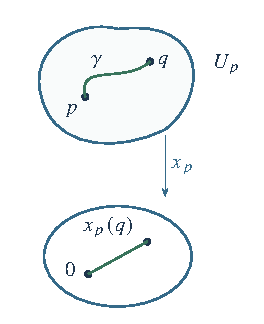
\includegraphics[width=.38\textwidth]{m3-fig-05.pdf}
 \FigureTag{M3.5}{fig:m3-fig-05}
\end{figure}
% Source page 5
By the Fundamental Theorem of Calculus,
$\frac{dz_p}{dx_p}(x_p(q))=\phi_p(x_p(q))$.
Define $\widetilde z_p:=z_p\circ x_p$. Then $\omega=d\widetilde z_p$.
Equivalently, $\widetilde z_p$ is obtained by integrating the local coefficient $\phi_{x_p}\circ x_p$.
But we notice that
\[
 \frac{d\widetilde z_p}{d\widetilde z_q}=1
 \quad\Longrightarrow\quad
 \widetilde z_p=\widetilde z_q+c
 \qquad\text{(translation charts).}
\]


% Source page 7
Now consider the space
$\Omega M_g:=\{(X,\omega):\omega\in\Omega X,\ \omega\ne0\}$.
The projection $\Omega M_g\xrightarrow{\pi}M_g$ is the complement of the zero section in a holomorphic vector bundle of rank $g$, since $\dim\Omega X=g$. A \emph{stratum} is
\[
 \Omega M_g(p_1,\ldots,p_n)
 :=\{(X,\omega):(\omega)=p_ix_i,\ x_i\in X,\ p_i\ge0\}
 \subset\Omega M_g.
\]
% Author check: the divisor expression has no summation sign in the source.
\subsection{\texorpdfstring{$\SL_2(\mathbb R)$}{SL2(R)} Action}
Let $(X,\omega)\in\Omega M_g$. We have a translation structure
$(U_p,\widetilde z_p)$ on $X$. For $A\in\SL_2(\mathbb R)$, define
$A\cdot(X,\omega):=(U_p,A\circ\widetilde z_p)$. Then
\[
 \begin{aligned}
 (A\circ\widetilde z_q)\circ(A\circ\widetilde z_p)^{-1}(z)
 &=A\circ(\widetilde z_q\circ\widetilde z_p^{-1})(A^{-1}(z))\\
 &=A(A^{-1}(z)+c)=z+A(c).
 \end{aligned}
\]
Thus $\SL_2(\mathbb R)\curvearrowright\Omega M_g$ by stretching and
rotating the translation structure.
% Source page 8
\begin{remark}
$(M_g,\operatorname{Re}(\widetilde\omega_{\mathrm{WP}}))$ is a highly
inhomogeneous space:
$(T_XM_g,|\cdot|_{\mathrm{WP}})\not\cong(T_YM_g,|\cdot|_{\mathrm{WP}})$
for $X\ne Y$. Thus $\Omega M_g$ is a bundle of nonzero holomorphic forms over $M_g$.
The space $\Omega M_g$ admits an $\SL_2(\mathbb R)$ action and is therefore
highly homogeneous. One can easily observe that $\SL_2(\mathbb R)$
preserves $\Omega M_g(p_1,\ldots,p_n)$.
\end{remark}
% Author check: the tangent-space comparison and homogeneity claim are retained.
If $A\in\operatorname{SO}_2(\mathbb R)$, that is, a rotation, then
$A\cdot(X,\omega)$ is just $(X,e^{i\theta}\omega)$. We thus have
\begin{figure}[H]
 \centering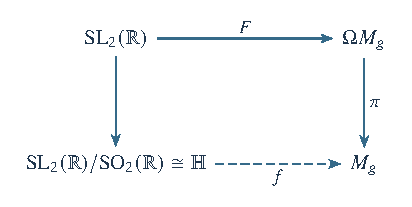
\includegraphics[width=.64\textwidth]{m3-fig-08.pdf}
 \FigureTag{M3.8}{fig:m3-fig-08}
\end{figure}
Here $F(A):=A\cdot(X,\omega)$ for some fixed $(X,\omega)\in\Omega M_g$.
The map $\pi\circ F$ factors through
$\SL_2(\mathbb R)/\operatorname{SO}_2(\mathbb R)$.
The action $\SL_2(\mathbb R)\curvearrowright\mathbb H$ is by fractional
linear transformations, with
$\operatorname{Stab}(i)=\operatorname{SO}_2(\mathbb R)$ and
$\operatorname{Orb}(i)=\mathbb H$.
% Source page 9

\paragraph{Geodesic rays in $M_g$.}
Every point has a real geodesic through it. For fixed $(X,\omega)$, set
\[
 \gamma\colon[0,\infty)\to M_g,\qquad
 \gamma(t):=\begin{pmatrix}e^{-t}&0\\0&e^t\end{pmatrix}\cdot(X,\omega).
\]
\begin{figure}[H]
 \centering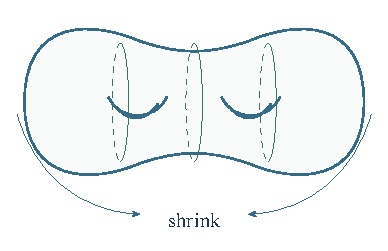
\includegraphics[width=.55\textwidth]{m3-fig-09.pdf}
 \FigureTag{M3.9}{fig:m3-fig-09}
\end{figure}
\paragraph{Teichm\"uller curves in $M_g$.}
Let $\operatorname{Stab}(X,\omega)=:\SL(X,\omega)$, the \emph{Veech group}.
Then
\[
 \SL(X,\omega)\curvearrowright
 \SL_2(\mathbb R)/\operatorname{SO}_2(\mathbb R)\cong\mathbb H.
\]
If $\SL(X,\omega)$ were a lattice in $\SL_2(\mathbb R)$, then the
normalisation map
$V\cong\mathbb H/\SL(X,\omega)\longrightarrow M_g$
would define a Teichm\"uller curve in $M_g$ generated by $(X,\omega)$.
% Source page 10

% Source page 11
\setcounter{theorem}{8}\begin{proposition}
$\SL(X,\omega)$ is a discrete subgroup of $\SL_2(\mathbb R)$, and the
quotient is never compact.
\end{proposition}
\begin{proof}
$\SL(X,\omega)$ is discrete because, for $g\in\SL_2(\mathbb R)$ close
 to $\id$, $\operatorname{dilatation}(g)=1$ if and only if
 $g\in\operatorname{SO}_2(\mathbb R)$, but
 $\operatorname{SO}_2(\mathbb R)$ does not preserve $\SL(X,\omega)$.
 $\SL(X,\omega)$ is not cocompact, because otherwise
 \[
 \SL_2(\mathbb R)/\SL(X,\omega)\cong
 \SL_2(\mathbb R)\cdot(X,\omega)=\operatorname{Orb}(X,\omega)
 \]
 would be compact, but
 \[
 \left(g_t=\begin{pmatrix}e^{-t}&0\\0&e^t\end{pmatrix}\right)
 \cdot(X,\omega)\xrightarrow{\pi}X_t
 \]
 is noncompact in $M_g$.
 % Author check: the source's abbreviated discreteness and noncompactness arguments are retained.
\end{proof}
\paragraph{Remarks.}
\begin{enumerate}
 \setcounter{enumi}{0}\item If $\omega\in\Omega X$, then in a chart $(U_p,x_p)_p$,
 $\omega=\phi_{x_p}\,dx_p$. Hence
 $\phi_{x_p}\frac{dx_p}{dx_q}=\phi_{x_q}$.
 In $(U_p,\widetilde z_p)$, we have $\phi_{x_p}\equiv1$ for
 $p\in X\setminus\Sigma$. Thus
 $\frac{d\widetilde z_p}{d\widetilde z_q}=1$, so
 $\widetilde z_p=\widetilde z_q+c$.

\end{enumerate}
% Source page 13 (continuation of the preceding remarks).
\begin{figure}[H]
 \centering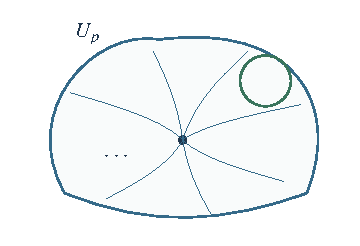
\includegraphics[width=.48\textwidth]{m3-fig-12.pdf}
 \FigureTag{M3.12}{fig:m3-fig-12}
\end{figure}
We have $\frac{d\phi}{d\widetilde z_p}=1$, so $\phi=\widetilde z_p+c$.
\begin{enumerate}[start=3]
 \setcounter{enumi}{2}\item \textbf{Twisted action of the Veech group.}
 The fractional linear action $\SL_2(\mathbb R)\curvearrowright\mathbb H$
 gives
 $\SL_2(\mathbb R)/\operatorname{SO}_2(\mathbb R)\cong\mathbb H$,
 by $A\mapsto A\cdot i$. The linear action
 $\SL_2(\mathbb R)\curvearrowright\mathbb R^2\cong\mathbb C$ gives
 \[
 \operatorname{SO}_2(\mathbb R)\backslash\SL_2(\mathbb R)\cong\mathbb H,
 \qquad A\longmapsto\frac{A(i)}{A(1)}.
 \]
 As $\SL_2(\mathbb R)$-spaces,
 $\SL_2(\mathbb R)/\operatorname{SO}_2(\mathbb R)$ and
 $\operatorname{SO}_2(\mathbb R)\backslash\SL_2(\mathbb R)$ are isomorphic.
 With respect to the second action, $\SL(X,\omega)$ is discrete.
 The map between the two quotient spaces is $A\mapsto A^{-1}$; on
 $\mathbb H$ it is $t\mapsto-\overline t$.
 % Source page 14
 One conjugates the linear action of $\SL(X,\omega)$ on $\mathbb H$
 by $t\mapsto-\overline t$ to make it fractional linear.
 Thus $\mathbb H/\SL(X,\omega)\longrightarrow M_g$ is a Teichm\"uller curve.
 \setcounter{enumi}{3}\item Define
 \[
 \begin{split}
 \operatorname{Aff}^+(X,\omega):=\{\phi\colon X\to X:\;&
 \phi\in\operatorname{Diff}^+(X),\
 \phi(Z(\omega))=Z(\omega),\\
 &\text{locally }\phi(x,y)=A\binom xy+b,\quad A\in\SL_2(\mathbb R)\}.
 \end{split}
 \]
 \begin{figure}[H]
  \centering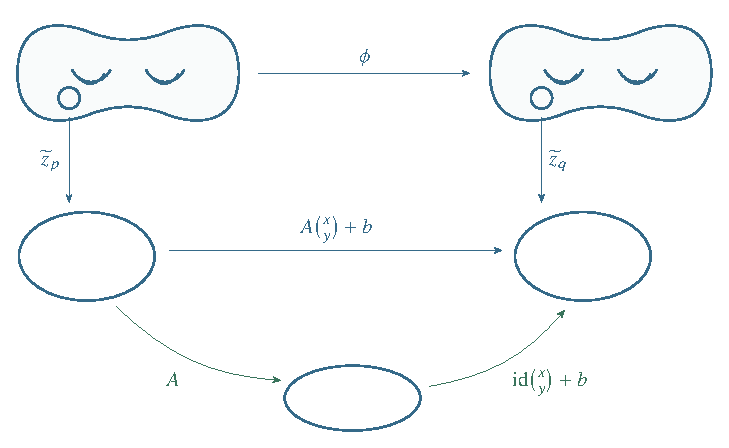
\includegraphics[width=.84\textwidth]{m3-fig-13.pdf}
  \FigureTag{M3.13}{fig:m3-fig-13}
 \end{figure}
 Then $D\phi=A$, so
 $A\cdot(X,\omega)=(U_p,A\circ\widetilde z_p)=(X,\omega)$.
 We obtain
 $\operatorname{Aff}^+(X,\omega)\xrightarrow{D}\SL(X,\omega)\to1$;
 the identity map gives surjectivity.
 We have $A=\id$ if and only if
 \[
 \phi\in\Aut(X,\omega):=
 \{\phi\colon X\to X:\phi\in\Aut(X),\ \phi^*\omega=\omega\}.
 \]
 % Source page 15
 By Hurwitz's theorem, for $g>1$, $|\Aut(X,\omega)|<84(g-1)$.
 Thus
 \[
 1\longrightarrow\Aut(X,\omega)\lhook\joinrel\longrightarrow
 \operatorname{Aff}^+(X,\omega)\xrightarrow{D}\SL(X,\omega)
 \longrightarrow1.
 \]
 For $g>1$, $\SL(X,\omega)$ is virtually the affine symmetry group.
 % Author check: the strict Hurwitz inequality is retained.
 \setcounter{definition}{5}\begin{definition}[Primitive Teichm\"uller curve]
 $(X,\omega)$ is said to be primitive if there is no $f\colon X\to Y$
 such that $f^*\eta=\omega$ with $\eta\in\Omega Y$.
 A Teichm\"uller curve generated by a primitive curve
 $(X,\omega)\in\Omega M_g$ is a \emph{primitive Teichm\"uller curve}.
 \end{definition}
 % Author check: the source does not exclude isomorphisms or the identity in this definition.
 If $(X,\omega)$ is primitive, then $\Aut(X,\omega)=\{\id\}$.
 Hence $\SL(X,\omega)\cong\operatorname{Aff}^+(X,\omega)$.

\end{enumerate}
% Source page 16
\subsection{Summary}
\begin{enumerate}
 \setcounter{enumi}{0}\item $\operatorname{Re}(\widetilde\omega_{\mathrm{WP}})$ descends to $M_g$.
 \setcounter{enumi}{1}\item Every $(X,\omega)\in\Omega M_g$ gives a translation structure.
 \setcounter{enumi}{2}\item $\SL_2(\mathbb R)\curvearrowright\Omega M_g$ stretches the translation structure.
 \setcounter{enumi}{3}\item Fix $(X,\omega)\in\Omega M_g$. We have the following diagram:
 where $F(A)=A\cdot(X,\omega)$ and $f$ is an isometric immersion.
 \begin{figure}[H]
  \centering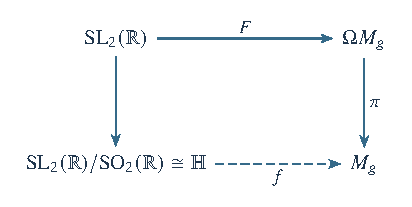
\includegraphics[width=.64\textwidth]{m3-fig-14.pdf}
  \FigureTag{M3.14}{fig:m3-fig-14}
 \end{figure}
 \setcounter{enumi}{4}\item The Veech groups $\operatorname{Stab}(X,\omega)=\SL(X,\omega)$
 are discrete and not cocompact.
 \setcounter{enumi}{5}\item If $\SL(X,\omega)$ is a lattice in $\SL_2(\mathbb R)$, we obtain
 Teichm\"uller curves $V\cong\mathbb H/\SL(X,\omega)\longrightarrow M_g$.
 \setcounter{enumi}{6}\item There is a twisted action of $\SL(X,\omega)$ on $\mathbb H$.
 \setcounter{enumi}{7}\item $\SL(X,\omega)\cong
 \operatorname{Aff}^+(X,\omega)/\Aut(X,\omega)$ is virtually the affine
 symmetry group for $g>1$.
\end{enumerate}
% Source page 17
\begin{enumerate}[start=9]
 \setcounter{enumi}{8}\item Define the \emph{trace field}
 $K:=\mathbb Q\{\operatorname{tr}(A):A\in\SL(X,\omega)\}\subset\mathbb R$.
 This is a totally real number field with $\deg(K/\mathbb Q)\le g$.
 Thus the trace field connects the geometry of Teichm\"uller curves with number theory.
 \setcounter{enumi}{9}\item A Teichm\"uller curve generated by $(X,\omega)$ has the following
 invariants:
 \begin{enumerate}[label=(\roman*)]
  \setcounter{enumii}{0}\item $\SL(X,\omega)$ is determined by $V\hookrightarrow M_g$ up to
  conjugacy, since $\SL(X,\omega)\cong\Deck(\mathbb H/V)$;
  \setcounter{enumii}{1}\item the trace field $K$;
  \setcounter{enumii}{2}\item the stratum to which $(X,\omega)$ belongs.
 \end{enumerate}
\end{enumerate}
\subsection{Broad Goals}
\begin{enumerate}
 \setcounter{enumi}{0}\item Understand the $\SL_2(\mathbb R)$ action on the strata
 $\Omega M_g(p_1,\ldots,p_n)$: ergodicity, equidistribution, and so on.
 \setcounter{enumi}{1}\item Classify $\SL(X,\omega)$ and $\mathbb H/\SL(X,\omega)$ when
 $\SL(X,\omega)$ is a lattice.
 \setcounter{enumi}{2}\item Understand the geometry of the strata of $\Omega M_g$.
\end{enumerate}

% Source page 18
\subsection{Billiards and Teichm\"uller Curves}
Let $P$ be a polygon with angles in $\mathbb Q\pi$, that is, rational
multiples of $\pi$, such that every edge is paired with another parallel edge of the same length.
\begin{figure}[H]
 \centering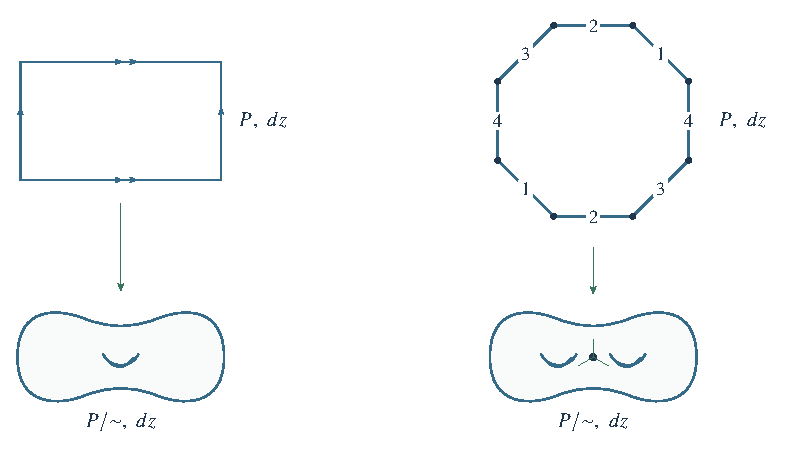
\includegraphics[width=.90\textwidth]{m3-fig-15.pdf}
 \FigureTag{M3.15}{fig:m3-fig-15}
\end{figure}
% Source page 19
This immediately gives a translation structure on $P/{\sim}$ because the
charts are given by translations away from singular points.
\begin{figure}[H]
 \centering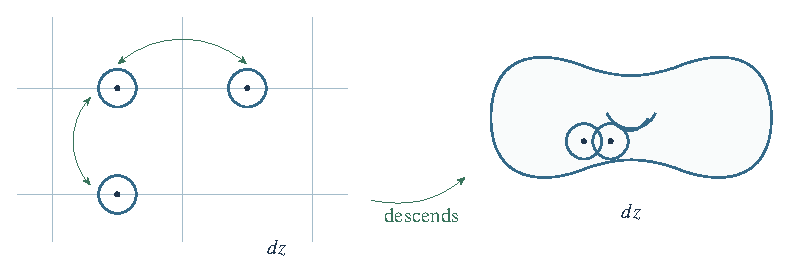
\includegraphics[width=.84\textwidth]{m3-fig-16.pdf}
 \FigureTag{M3.16}{fig:m3-fig-16}
\end{figure}
In general, $dz$ descends to a flat metric with cone singularities at
finitely many points. How many points? Say $k$.
Triangulating the surface, or equivalently the polygon, gives
\[
 \chi(X)=\chi(P/{\sim})=-(2g-2)=f-e+v,\qquad e=\frac32f.
\]
Thus $2-2g=f-\frac32f+v$, giving $f=(4g-4)+2v$.
The angle sum of each triangle is $\pi$, so the total angle sum is
$\pi f=(4g-4)\pi+2\pi v$.
% Source page 20
\setcounter{theorem}{9}\begin{proposition}
The angle at a cone singularity is a multiple of $2\pi$.
\end{proposition}
\begin{proof}
The cone angles of $P/{\sim}$ can be computed from the edge identifications.
\begin{figure}[H]
 \centering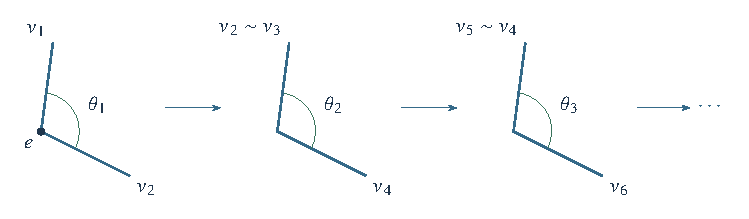
\includegraphics[width=.85\textwidth]{m3-fig-17.pdf}
 \FigureTag{M3.17}{fig:m3-fig-17}
\end{figure}
The cone angle at $e$ is $\sum_{i=1}^n\theta_i$. For every edge vector $v_i$ around the identified vertex, there is a parallel partner $v_j$. Returning to $v_1$ requires an integral number of full turns. Consequently
$2\pi\mid\sum_{i=1}^n\theta_i$.
\end{proof}
Let the cone angles be $2\pi(n_i+1)$ at $p_i$ in $P/{\sim}$. Then
\[
 2\pi\sum_{i=1}^k n_i=\pi f-2\pi k=(4g-4)\pi,
 \qquad 2\pi n_i=2\pi(n_i+1)-2\pi.
\]
Hence $\boxed{\sum_{i=1}^k n_i=2g-2}$.
% Author check: the source moves from v triangulation vertices to k cone points without explaining the choice.
% Source page 21
\subsection{From Translation Structure to Polygon}
\setcounter{theorem}{10}\begin{proposition}
Between any two singular points of a translation structure on $X$, there
is a geodesic in every homotopy class of arcs joining those points.
\end{proposition}
\begin{proof}
Let $[\gamma]$ be a homotopy class joining $p,q\in\Sigma$.
Break $\gamma(t)$ into finitely many segments, each in some local chart.
One can first construct a geodesic polygonal path joining $p$ and $q$,
as shown in the picture; call it $\widetilde\gamma$.
By construction, $\widetilde\gamma\in[\gamma]$, that is,
$\widetilde\gamma\sim\gamma$.
Now inductively straighten the polygonal path to a geodesic.
\begin{figure}[H]
 \centering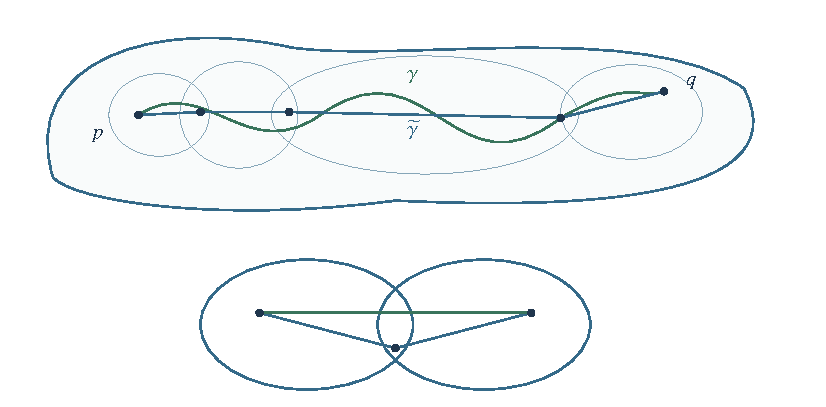
\includegraphics[width=.88\textwidth]{m3-fig-18.pdf}
 \FigureTag{M3.18}{fig:m3-fig-18}
\end{figure}
This proves the proposition.
\end{proof}
% Source page 22
This shows that we can triangulate the surface $X$ by joining singular
points. Therefore one obtains a polygonal representation.
\subsection{Billiards and Polygons}
\begin{figure}[H]
 \centering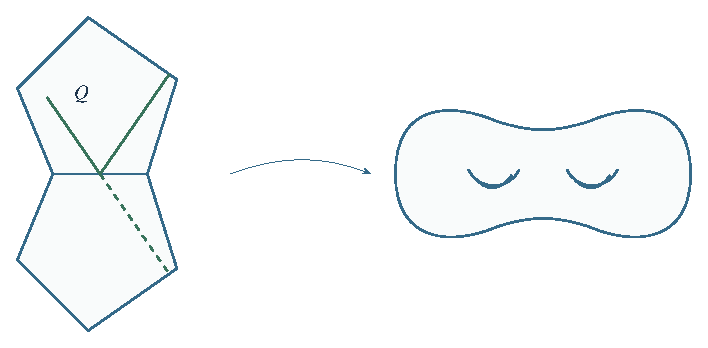
\includegraphics[width=.77\textwidth]{m3-fig-19.pdf}
 \FigureTag{M3.19}{fig:m3-fig-19}
\end{figure}
For background, see H. Masur, \emph{Rational Billiards and Flat Structures}.
Let $G_Q$ be the group generated by reflections along the sides.
Set $N=|G_Q|<\infty$. For $\theta\in S^1$, consider the orbit
$G_Q\cdot\theta=\{\theta_1,\ldots,\theta_{|G_Q|}\}
=\{\theta_1,\ldots,\theta_N\}$.
Consider $2N$ copies of $Q$. Pick a side $s$ of $Q_i$ and reflect
$\theta_i$ along $s$; it is $\theta_j$ for some $j\in\{1,\ldots,N\}$.
Glue the identical sides $s$ in $Q_i$ and $Q_j$.
% Author check: the source counts 2N copies after defining N=|G_Q| and uses reflection along sides without further qualification.
% Source page 23
The resulting object is a genus-$g$ surface with a flat metric having
cone singularities. We have
\[
 \operatorname{genus}(P/{\sim})
 =1+\frac N4\left(k-2-\sum_{i=1}^k\frac1{n_i}\right),
\]
where the angles of the billiard $k$-gon are $\pi m_i/n_i$,
for $i=1,\ldots,k$.
\subsection{Billiard Dynamics}
\begin{figure}[H]
 \centering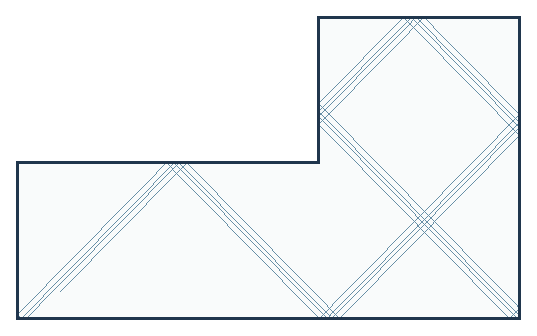
\includegraphics[width=.69\textwidth]{m3-fig-20.pdf}
 \FigureTag{M3.20}{fig:m3-fig-20}
\end{figure}
\paragraph{Topologically optimal.}
Every trajectory $\gamma(t)$ is dense or periodic.
\paragraph{Ergodically optimal.}
Every trajectory $\gamma(t)$ is periodic or equidistributed:
\[
 \underbrace{\lim_{T\to\infty}\frac1T\int_0^T f(\gamma(t))\,dt}_{\text{time average}}
 =
 \underbrace{\frac1{\Area(P)}\int_P f(z)|dz|^2}_{\text{space average}}.
\]
For background, see L. DeMarco, \emph{Conformal Geometry of Billiards}.
\paragraph{Polygonal lattice.}
If $(X,\omega)$ is obtained from $P$ by unfolding and $\SL(X,\omega)$
is a lattice, we call $P$ a polygonal lattice.
\[
 \text{polygonal lattice}\Longrightarrow\text{ergodically optimal}
 \Longrightarrow\text{topologically optimal}.
\]
% Source page 24

Thus billiard dynamics gives us curves in $M_g$.
In genus $2$, examples arise from the pentagon, octagon, and decagon.
\setcounter{theorem}{12}\begin{theorem}[McMullen]
If $\operatorname{genus}(X)=2$, then the following are equivalent:
$(X,\omega)$ is ergodically optimal; $(X,\omega)$ is topologically optimal;
and $\SL(X,\omega)$ is a lattice.
\end{theorem}
% BLOG-CONTENT-END
\end{document}
